\section{Goal}
% TODO What is the problem and why do we care
    \subsection{Goal}
        \begin{frame}
            \frametitle{Goal}
                 \begin{itemize}
                    \item Reduce the efforts required to build MSR tools
                    \item Ease the process of adopting, customizing and sharing MSR tools
                    \item Allow users to run third-party tools more securely
                 \end{itemize}

            %\begin{figure}
            %\centering
            %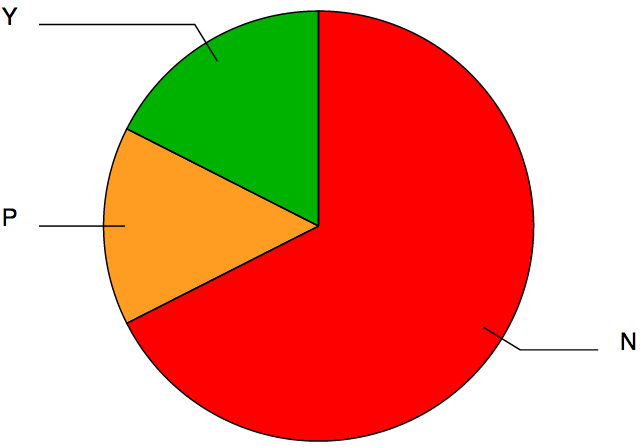
\includegraphics[width=0.55\linewidth]{figures/toolsavailability}
            %\end{figure}
        \end{frame}

        \subsection{Why Important?}
        \begin{frame}
            \frametitle{Scenario 1: MSR Tool Building and Sharing}
        User wants to build a tool for Association Mining
        %    Build    a tool for mining the source code, version data, and bugs
            \begin{columns}
                \column{0.65\textwidth}
                    \begin{itemize}
                      \item Source code
                          \begin{itemize}
                            \item Java source code
                          \end{itemize}
                      \item Version control systsm(VCS)
                          \begin{itemize}
                            \item GIT
                          \end{itemize}
                      \item Bug Information
                          \begin{itemize}
                            \item Github-Issues Bug Tracker
                          \end{itemize}
                    \end{itemize}

                \column{0.35\textwidth}
                    \begin{figure}
                    \centering
                    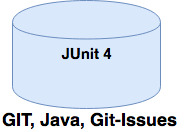
\includegraphics[width=0.60\linewidth]{figures/junit4.jpg}
                    \caption{\tiny{Software Repository Data}}
                    \end{figure}

            \end{columns}
        \end{frame}

        \begin{frame}
            \frametitle{Scenario 1: Tool Building and Sharing}
            Build a tool for association mining
            \begin{figure}
                \centering
                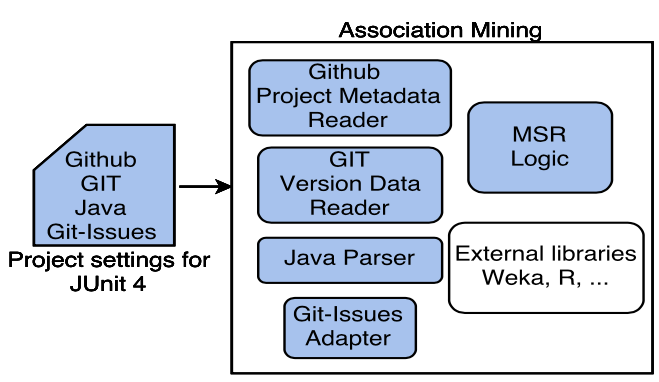
\includegraphics[width=0.60\linewidth]{figures/association.png}
                \caption{Association Minging Tool Details}
            \end{figure}
        \end{frame}

        \begin{frame}
            \frametitle{Scenario 1: Tool Building and Sharing}
            Share the built tool with other researchers and practitioners
            \begin{figure}
                \centering
                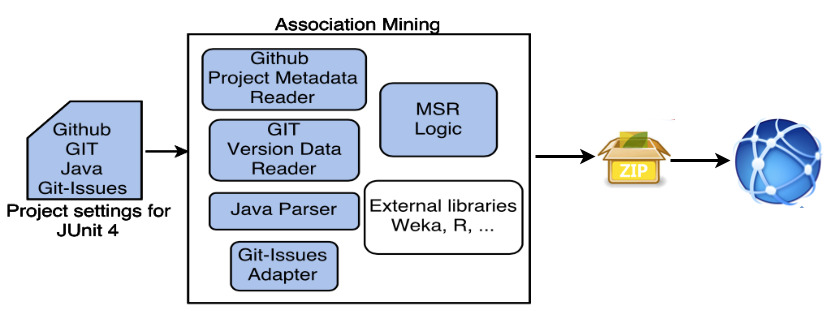
\includegraphics[width=0.85\linewidth]{figures/junitsharing.jpg}
                \caption{Complete process of building and sharing tool}
            \end{figure}
        \end{frame}

        \begin{frame}
            \frametitle{Scenario 2: Adopting a shared tool}
            \begin{figure}
                \centering
                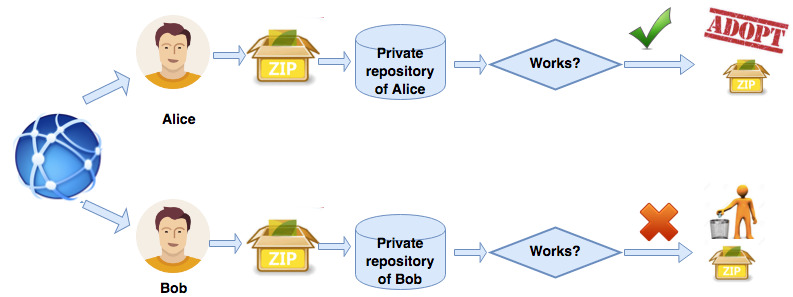
\includegraphics[scale=0.35]{figures/adopting.jpg}
                \caption{Repository Mining Tool Building}
            \end{figure}
        \end{frame}

%\begin{comment}
        \begin{frame}
            \frametitle{Scenario 2: Adopting a shared MSR tool}
             \centering
                Why Bob is not able to adopt the same tool? \\
                \& \\
                What are the possible points of failure?
        \end{frame}
%\end{comment}

        \begin{frame}
            \frametitle{How MSR tools are build?}
            \begin{itemize}
                \item MSR tools are build for specific project setting.
                \item A project setting defines types and sources of various MSR artifacts
            \end{itemize}
        \end{frame}

                \begin{frame}
                    \frametitle{How MSR tools are build?}
                    \begin{itemize}
                        \item MSR tools are build for specific project setting.
                        \item A project setting defines types and sources of various MSR artifacts
                        \item MSR Artifacts: Any kind of information realted to your software
                        \begin{itemize}
                            \item Revision history from version control system (VCS)
                            \item Source code of programming language(s)
                            \item Bug data from bug trackers
                            \item Project metadata
                            \item users and teams data from forges
                        \end{itemize}
                    \end{itemize}
                \end{frame}

        \begin{frame}
            \frametitle{Association Mining Tool Challenges}
            \begin{columns}
            %    Build    a tool for mining the source code, version data, and bugs
                \column{0.5\textwidth}
                \begin{itemize}
                    \item User is required to build necessary data preparation tools
                 \end{itemize}
                \column{0.65\textwidth}
                 \begin{figure}
                    \centering
                        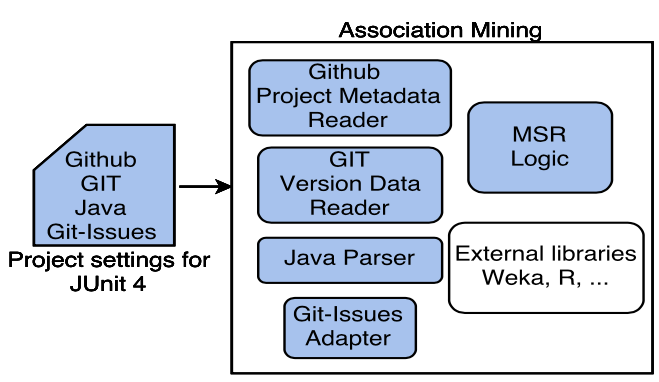
\includegraphics[width=0.85\linewidth]{figures/association.png}
     %                       \caption{Software Repository Data}
                 \end{figure}
             \end{columns}
        \end{frame}

        \begin{frame}
            \frametitle{Association Mining Tool Challenges}
            \begin{columns}
            %    Build    a tool for mining the source code, version data, and bugs
                \column{0.5\textwidth}
                \begin{itemize}
                    \item User is required to build necessary data preperation tools
                    \item Tool are tightly coupled with SCM systems
                 \end{itemize}
                \column{0.65\textwidth}
                 \begin{figure}
                    \centering
                        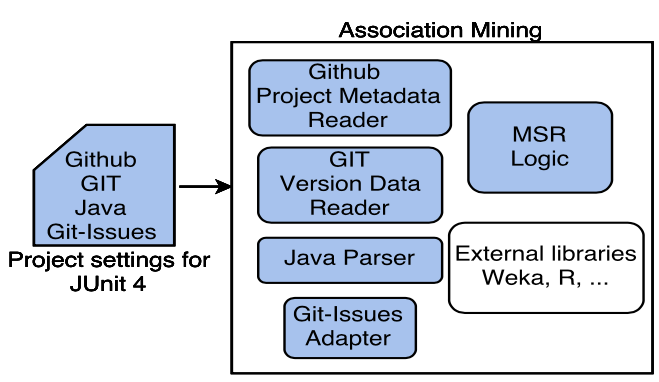
\includegraphics[width=0.85\linewidth]{figures/association.png}
     %                       \caption{Software Repository Data}
                 \end{figure}
             \end{columns}
        \end{frame}


        \begin{frame}
            \frametitle{Potential Points of failure}
            \begin{alertblock}{Failure Cause}
                An MSR tool build for one project setting may not work for different project settings.
            \end{alertblock}
             \begin{figure}
                \centering
                    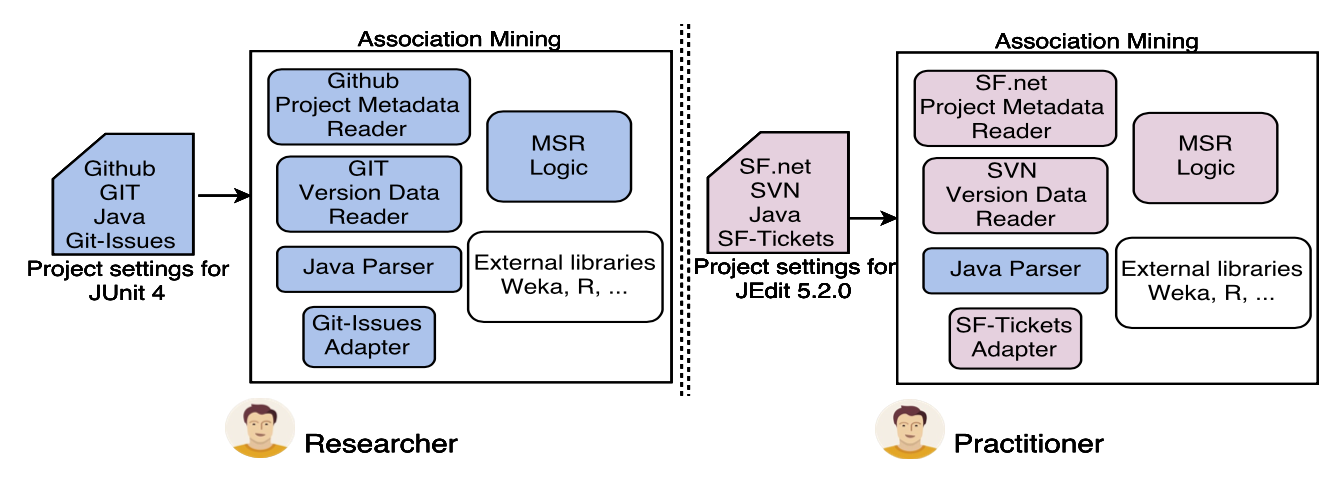
\includegraphics[width=0.85\linewidth]{figures/adoptingreserch.png}
                        \caption{A scenario of a practitioner adopting a MSR tool built by a researcher.}
             \end{figure}
        \end{frame}

\begin{comment}
        \begin{frame}
            \frametitle{Failure: Mismatched Project Settings}
             %    Build    a tool for mining the source code, version data, and bugs
             \begin{columns}
                \column{0.33\textwidth}
                    \centering Tool
                    \begin{figure}
                        \centering
                        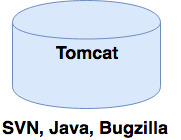
\includegraphics[width=0.45\linewidth]{figures/tomcat.jpg}
 %                       \caption{Software Repository Data}
                    \end{figure}

                \column{0.33\textwidth}
                    \centering Alice
                    \begin{figure}
                        \centering
                        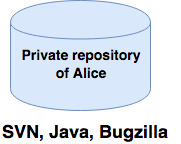
\includegraphics[width=0.45\linewidth]{figures/privaterepo.jpg}
%                        \caption{Software Repository Data}
                    \end{figure}

                \column{0.33\textwidth}
                    \centering Bob
                    \begin{figure}
                        \centering
                        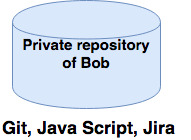
\includegraphics[width=0.45\linewidth]{figures/privaterepobob.jpg}
%                        \caption{Software Repository Data}
                    \end{figure}
             \end{columns}
        \end{frame}

    \subsection{A study of reusability of MSR tools}
        \begin{frame}
            \frametitle{Reusability of published MSR tools\footnote{\label{replicability}{Replicating MSR:A study of the potential replicability of papers, Gregorio Robles et.al,  MSR 2010}}}
            \begin{columns}
                \column{0.55\textwidth}
                    \centering
                        \begin{itemize}
                            \item Y = Replicable
                            \item N = Not replicable
                            \item P = Partially replicable
                        \end{itemize}

                \column{0.45\textwidth}
                    \centering
                    \begin{figure}
                        \centering
                        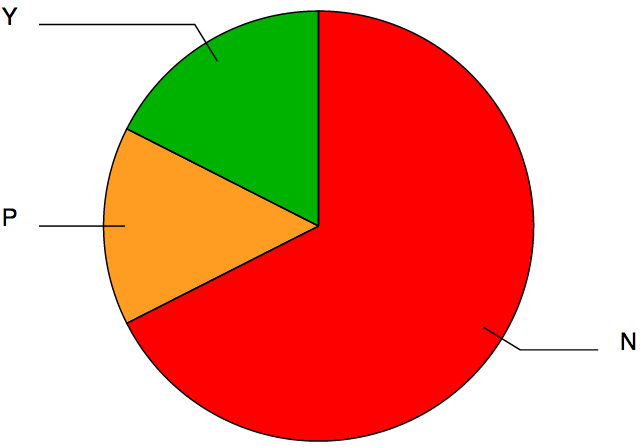
\includegraphics[width=0.75\linewidth]{figures/toolsavailability.png}
                        \caption{Replicability of $MSR^{3}$}
                    \end{figure}
            \end{columns}
        \end{frame}

\end{comment}

        \begin{frame}
            %\frametitle{Challenges: Scenario 1 MSR Tool Building and Sharing}
        %    Build    a tool for mining the source code, version data, and bugs
             \centering
             How to make adopting MSR tools possible?
        \end{frame}